\chapter{ANALYSIS}
\label{chap:analysis}
The analysis is optimized to maximize the significance of the final Higgs Boson selected events. 
All events are separated into five categories, three of which are designed to select events associated with the SM Higgs Boson production mechanisms, while the remaining two are tailored to select events associated with neutral MSSM Higgs Boson production mechanisms. 
The separation of the analysis into five separate categories will provide an increased significance in the final result when combined. 
The advantages of the event categorization will be discussed in more detail in Chapter \ref{chap:results}.
Due to the high number of interactions, the first step in the selection of the candidate Higgs boson events is to ensure an efficient trigger path exists to filter signal events from common events, often referred to as minimum bias events.
To protect against additional sources of energy deposits and charged tracks arising from pile-up, a primary vertex with the highest $p_{T}$ sum is selected. 
All charged particles are checked for compatibility with the selected primary vertex.
Once the primary vertex has been selected, high quality muon and tau candidates are selected.
%Once the events have been stored the analysis begins by selecting high quality muon and tau candidates existing in the event.
%Once the muons and taus have been selected a common primary vertex is identified to protect against possible pile-up interference.
The muon, tau objects, and any missing transverse energy are then combined into a composite object that would represent decay products of the originating Higgs Boson.
Finally, additional kinematic variables are used to reject possible backgrounds from $W \rightarrow \mu \nu$, QCD multi-jet, and $Z\rightarrow\mu\mu$ events.

\section{Trigger Selection}
\label{sec:triggerselection}
As discussed in Section \ref{sec:triggersystem} the majority of data coming from the detector is discarded. 
For this reason it is important that an appropriate trigger path exists for any analysis.
For this analysis a number of muon + hadronic tau cross triggers are used to filter the data coming from the detector.
The cross trigger uses a combination of an isolated muon trigger along with an isolated tau trigger.
Where possible the trigger used is the lowest possible transverse momentum ($p_{T}$) combination that remains unprescaled.
For this reason the trigger $p_{T}$ thresholds used change for different run ranges and scale with the luminosity being delivered to the CMS detector.
Towards the end of the 2011 data taking an additional requirement on the muon pseudo-rapidity was added.
The primary driving force in the choice of $p_{T}$ cuts outlined in Section \ref{sec:particleselection} is the rising edge of the trigger efficiency close to the $p_{T}$ threshold of the trigger object, the treatment of the trigger efficiency will be discussed in Chapter \ref{chap:systematics}.
The specific triggers used in the analysis consist of an isolated muon, in most cases with $p_{T} > 15$ GeV, combined with a loosely isolated particle flow tau object with $p_{T} > 10$ GeV, $p_{T} > 15$ GeV, or $p_{T} > 20$ GeV, depending on the luminosity.

\begin{table}[tpb]
  \setlength{\capwidth}{0.9\textwidth}
  \begin{small}
  \begin{center}
    \caption{HLT TRIGGER PATHS USED}
    \label{tab:triggerpaths}
    \begin{tabular}{lcc}
      \toprule
      HLT Trigger Path & Run Range & Int. Luminosity [$fb^{-1}$] \\
      \midrule
      HLT\_IsoMu12\_LooseIsoPFTau10 		& 160431-163869 & 0.017 \\
      HLT\_Mu15\_LooseIsoPFTau20    		& 160431-163869 & 0.017 \\
      HLT\_IsoMu15\_LooseIsoPFTau15 		& 165088-178420 & 1.97 \\  
      HLT\_IsoMu15\_eta2p1\_LooseIsoPFTau20 	& 173236-180252 & 2.46 \\
      \bottomrule
    \end{tabular}
  \end{center}
  \end{small}
\end{table}



\section{Particle Selection}
\label{sec:particleselection}

\subsection{Primary Vertex Selection}
\label{sec:vertexselection}
Reconstructed vertices are selected based on a set of parameters to ensure that the vertex is of high quality.
The position of the vertex in the z-axis is required to lie in the range $-24 < z < 24$ cm and within $2$ cm in the transverse plane, both with respect to the nominal interaction point. 
The vertex with the highest $p_{T}$ sum of all associated tracks is then chosen as the primary vertex with respect to the following particle selection.
The vertex selection is summarized in Table \ref{tab:vertexselection}.

\begin{table}[htpb]
  \setlength{\capwidth}{0.9\textwidth}
  \begin{small}
  \begin{center}
    \caption{VERTEX SELECTION}
    \label{tab:vertexselection}
    \begin{tabular}{lcc}
      \toprule
      Cut Name & Requirement \\
      \midrule
      $z$     & $-24 < z < 24$ cm \\
      $r$     & $r < 2$ cm \\ 
      $p_{T}$ & $p_{T}^{max}$ \\
      \bottomrule
    \end{tabular}
  \end{center}
  \end{small}
\end{table}


\subsection{Muon Selection}
\label{sec:muonselection}
The $p_{T}$ of the muon is required to be greater than $17$ GeV to ensure that the selected muon will be associated with a sufficient trigger acceptance.
To ensure that the muon falls within the fiducial region of the muon system, the muon is required to fall within a pseudo-rapidity range of $-2.1 < \eta < +2.1$.
Muons are required to have associated tracks reconstructed in both the inner tracker and muon systems. 
After satisfying the acceptance requirements of $p_{T}$, $\eta$ and matching tracks, the muon kinematic distributions can be seen in the left hand side of Figure \ref{fig:muoncuts}
To ensure that the inner track is well reconstructed, the track is required to have at least one valid reconstructed hit in the inner pixel tracker as well as at least one valid reconstructed hit in the outer silicon strip tracker. 
A similar requirement is applied to the track in the muon system as it is required to have at least one valid hit. 
To ensure that the tracks from the inner tracker and muon system are well matched the global fit is required to have a maximum $\chi^{2}/DOF$ of 10. 
The transverse impact parameter ($d_{0}$) is required to be less than $0.045$ cm as measured with respect to the selected primary vertex.
\begin{figure}[ht]
\centering
\includeleptoncutplot{leptonSelection}{04_afterEvtSelMuonPt_beforeEvtSelTauAntiOverlapWithMuonsVeto}{muon}{Pt}{log}
\includeleptoncutplot{leptonSelection}{10_afterEvtSelMuonTrkIP_beforeEvtSelTauDecayModeFinding}{muon}{Pt}{log}

\includeleptoncutplot{leptonSelection}{04_afterEvtSelMuonPt_beforeEvtSelTauAntiOverlapWithMuonsVeto}{muon}{Eta}{linear}
\includeleptoncutplot{leptonSelection}{10_afterEvtSelMuonTrkIP_beforeEvtSelTauDecayModeFinding}{muon}{Eta}{linear}
\caption{$p_{T}$ (top) and $\eta$ (bottom) distributions for muons after acceptance cuts (left) and after isolation and identification (right).}
\label{fig:muoncuts}
\end{figure}

Muons are often produced in heavy quark decays which would arise from QCD multi-jet events. 
Such events would present a very large background. 
To combat this effect muons are required to be well isolated from other tracks and measured energy in the calorimeters.
To ensure that the muon is well isolated an isolation variable is calculated by summing the $p_{T}$ of other particle candidates that meet the following requirements:
\begin{itemize}
\item Several different tracking algorithms are used in the event reconstruction. As such tracks that may be compitable with the muon are excluded from the isolation sum. This prevents the muon itself from accidentily being included.
%\item The track of any additional candidate to be considered is compared to the track of the muon to ensure that the muon itself is excluded from the isolation sum. 
\item Isolation candidates are required to have a track compatible with the selected vertex.
\item Isolation candidates must fall within an isolation cone defined by a radius of $0.4$ in $\eta$-$\phi$ space around the muon.
\item Charged candidates are only considered if the candidate's $p_{T}$ is greater than $1$ GeV and the candidate does not lie within a veto-cone of radius $0.001$ around the muon.
\item All neutral and photon candidates are included in the isolation sum regardless of their $p_{T}$, however, these candidates are excluded if they lie within a veto-cone of radius $0.01$ around the muon.
\end{itemize}
In addition to the previously defined isolation sum, a correction ($\Delta\beta$) is applied to account for energy left by additional neutral particles associated with pile-up affects.
The $\Delta\beta$ correction is calculated by summing the $p_{T}$ of any charged candidates within the isolation cone that do not meet the primary vertex selection.
This $p_{T}$ sum is then corrected with a ratio of 2:1 to account for the average number of neutral candidates with respect to the charged candidates.
The final isolation sum is then calculated by summing the $p_{T}$ of the charged candidates, the $E_{T}$ of the neutral and photon candidates with the $\Delta\beta$ correction being subtracted from the sum if it is positive.
A relative isolation for the muon is calculated by taking the ratio of the isolation sum to the $p_{T}$ of the muon as shown in:
\begin{equation}
I_{rel} = \frac{\Sigma p_{T}(charged) + \Sigma E_{T}(neutral) + \Sigma E_{T}(photon) - \max(0,\Delta\beta)}{p_{T}(muon)}
\end{equation}
Kinematic distributions for muons satisfying identification and isolation requirements can be seen in the right hand side of Figure \ref{fig:muoncuts}.

\begin{table}[tpb]
  \setlength{\capwidth}{0.9\textwidth}
  \begin{small}
  \begin{center}
    \caption{MUON SELECTION}
    \label{tab:muonselection}
    \begin{tabular}{lcc}
      \toprule
      Cut Name & Requirement \\
      \midrule
      Transverse Momentum & $p_{T} > 17$ GeV \\
      Pseudo-rapidity & $-2.1 < \eta < 2.1$ \\
      Global Muon & Inner Track matching muon track \\
      $\chi^{2}$ & $\chi^{2}/DOF < 10$ \\
      Impact parameter & $d_{0} < 0.045$ cm \\
      Relative Isolation & $I_{rel} < 0.3$ \\
      \bottomrule
    \end{tabular}
  \end{center}
  \end{small}
\end{table}


\subsection{Tau Selection}
\label{sec:tauselection}
In order to ensure that the selected taus are also within the high efficiency range of the trigger they are required to have a $p_{T} > 20$ GeV and are restricted to a range in pseudo-rapidity of  $-2.5 < \eta < 2.5$. 
This ensures that the selected tau is in the fiducial region of the tracker, while limiting background contributions from QCD events in the forward detector.
Kinematic distributions for the tau leptons after acceptance selection can be seen in the left hand side of Figure \ref{fig:taucuts}
The identification and isolation of tau candidates is done using the Hadron Plus Strips (HPS) algorithm\cite{HPS}.
This algorithm constructs a tau object by combining charged hadron particle flow candidates with particle flow photon candidates in $\eta$ strips around the charged hadrons.
Taus typically decay into a single charged hadron (one prong) along with an additional zero or more neutral pions, or into three hadrons (three prong).
The HPS tau is required to have one of the following decay modes:
\begin{itemize}
\item Single Hadron
\item Hadron Plus One Strip
\item Hadron Plus Two Strips
\item Three Hadrons
\end{itemize}
To discriminate HPS taus from other jet objects an isolation requirement is applied by summing the $p_{T}$ of charged hadron candidates and the $E_{T}$ of photon candidates in a cone of radius $0.5$ in $\eta$-$\phi$ space around the tau.
In order to discriminate taus from muons a dedicated discriminant is used such that the highest $p_{T}$ charged hadron track is required not to be reconstructed as a muon.
It is also required that the ratio of the associated energy left in the HCAL to the transverse momentum is greater than $0.2$, in order to veto against minimally ionizing particles in the case that the tau has only a single hadron. 
To discriminate tau candidates from electrons a multivariate analysis (MVA) based electron pre-identification is applied using the electron $E/p$ and other calorimeter information with respect to the leading track.
%The muon discriminant used is 
A final anti-overlap veto ($\Delta R > 0.3$) is applied to the selected tau to protect against the same hits in the tracker being reconstructed as both a charged hadron candidate and a muon track.
Kinematic distributions for the tau leptons after identification and isolation requirements can be seen in the right hand side of Figure \ref{fig:taucuts}.
\begin{figure}[ht]
\centering
\includeleptoncutplot{leptonSelection}{07_afterEvtSelTauPt_beforeEvtSelMuonVbTfid}{tau}{Pt}{log}
\includeleptoncutplot{leptonSelection}{14_afterEvtSelTauElectronVeto_beforeEvtSelDiTauCandidateForMuTauAntiOverlapVeto}{tau}{Pt}{log}

\includeleptoncutplot{leptonSelection}{07_afterEvtSelTauPt_beforeEvtSelMuonVbTfid}{tau}{Eta}{linear}
\includeleptoncutplot{leptonSelection}{14_afterEvtSelTauElectronVeto_beforeEvtSelDiTauCandidateForMuTauAntiOverlapVeto}{tau}{Eta}{linear}
\caption{$p_{T}$ (top) and $\eta$ (bottom) distributions for taus after acceptance cuts (left) and after particle identification and isolation (right).}
\label{fig:taucuts}
\end{figure}


\subsection{Jet Selection}
\label{sec:jetselection}
Jets are used in order to classify events into categories designed to differentiate between events arising from different Higgs production mechanisms. 
Jets are reconstructed using the particle flow candidates and the anti-$k_{T}$ algorithm\cite{ANTIKT} with an opening of $R = 0.5$. 
A series of jet cleaning and identification cuts are first applied to any selected jets, these cuts include:
\begin{itemize}
\item Neutral Hadron Fraction $< 0.99$
\item Neutral EM Fraction $< 0.99$
\item Number of Constituents $> 1$
\item Charged Hadron Fraction $> 0$
\item Charged Multiplicity $> 0$
\item Charged EM Fraction $< 0.99$
\end{itemize}
In order to exclude selected leptons from the jet selection, jets are required to be separated by a $\Delta R$ of at least 0.5 in $\eta$-$\phi$ space from any selected muon or tau.
In order to determine if a jet originated from a bottom quark, a B-Tag requirement is checked.
This is done using the Track Counting High Efficiency discriminant, tracks that have a value for this discriminant ($d_{TCHE} > 3.3$) are considered to be B-Tagged\cite{BTV_10_001}.

\subsection{Missing Transverse Energy}
\label{sec:metselection}
Neutrinos interact only weakly, as such they will not interact with any of the sub-detectors as described in Chapter \ref{chap:detector}.
Rather than direct detection the presence of neutrinos is inferred via the concept of missing transverse energy ($\met$).
To calculate the $\met$, the total transverse energy ($E_{T}$) of all particle flow candidates is summed.
The momentum of the incident partons will be nearly parallel with the beam pipe, as such the energy in the transverse plane is expected to be very nearly balanced.
If all transverse energy is not accounted for, the $E_{T}$ sum will be non-zero and the resulting $\met$ is calculated to make up the discrepancy.
The $\met$ is useful in discriminating against events with W bosons or $t\overline{t}$ pairs, and is used in calculating the di-tau invariant mass distribution.


\section{Event Selection}
\label{sec:eventselection}

\subsection{Di-tau Candidate Selection}
\label{sec:ditauselection}
Di-tau candidates are reconstructed from muons and taus with selections described in Sections \ref{sec:muonselection} and \ref{sec:tauselection} respectively.
The muon and tau objects are required to be separated by a distance $\Delta R > 0.5$ in $\eta$-$\phi$ space to ensure that they do not represent the same physical object.

To reject background events arising from the decay of a W boson, two variables are used, the transverse mass of the $\mu$+$\met$ system ($M_{T}$), and $\pzetadiff$.
To reject this background for the MSSM Higgs search, the kinematics of tau decays is leveraged in the use of $\pzetadiff$.
In di-tau signal events the neutrinos are expected to be nearly collinear with the associated visible decay products, thus the direction of the missing transverse energy would lie between the visible decay products.
In contrast, events in which a lepton is produced via a semi-leptonic W boson decay, and to a lesser extent $t\overline{t}$ events, this correlation does not exist.
An axis $\zeta$ is defined by bisecting the directions of the visible decay products, the momentum of the visible decay products is then projected onto this axis producing the observable $p_{\zeta}^{vis}$.
An additional observable $p_{\zeta}^{miss}$ is created by projecting the missing transverse energy vector onto the same bisecting axis $\zeta$.
A final observable $\pzetadiff$ is used to reject W background events, it is defined as:
\begin{equation}
\label{eqn:pzetadiff}
\pzetadiff = p_{\zeta}^{miss} -  1.5 p_{\zeta}^{vis}
\end{equation}

In the SM search, the Higgs decays will tend to have a softer $p_{T}$ spectrum leading to the decay products being less collimated.
For this reason in order to reject this background in SM Higgs search the transverse mass is used to discriminate against events which arise from the semi-leptonic decay of a W boson.
The transverse mass is defined as 
\begin{equation}
\label{eqn:mt}
   M_{T} = p_{T}^{\mu}\met\sqrt{1-cos\Delta\phi},
\end{equation}
where $\Delta\phi$ is the angle between the muon's momentum vector and the reconstructed $\met$.
The transverse mass is required to be less than $40$ GeV.
Both the transverse mass and $\pzetadiff$ distributions can be seen in Figure \ref{fig:mtpzeta}.

\begin{figure}[ht]
  \begin{minipage}[b]{0.5\linewidth}
\centering
  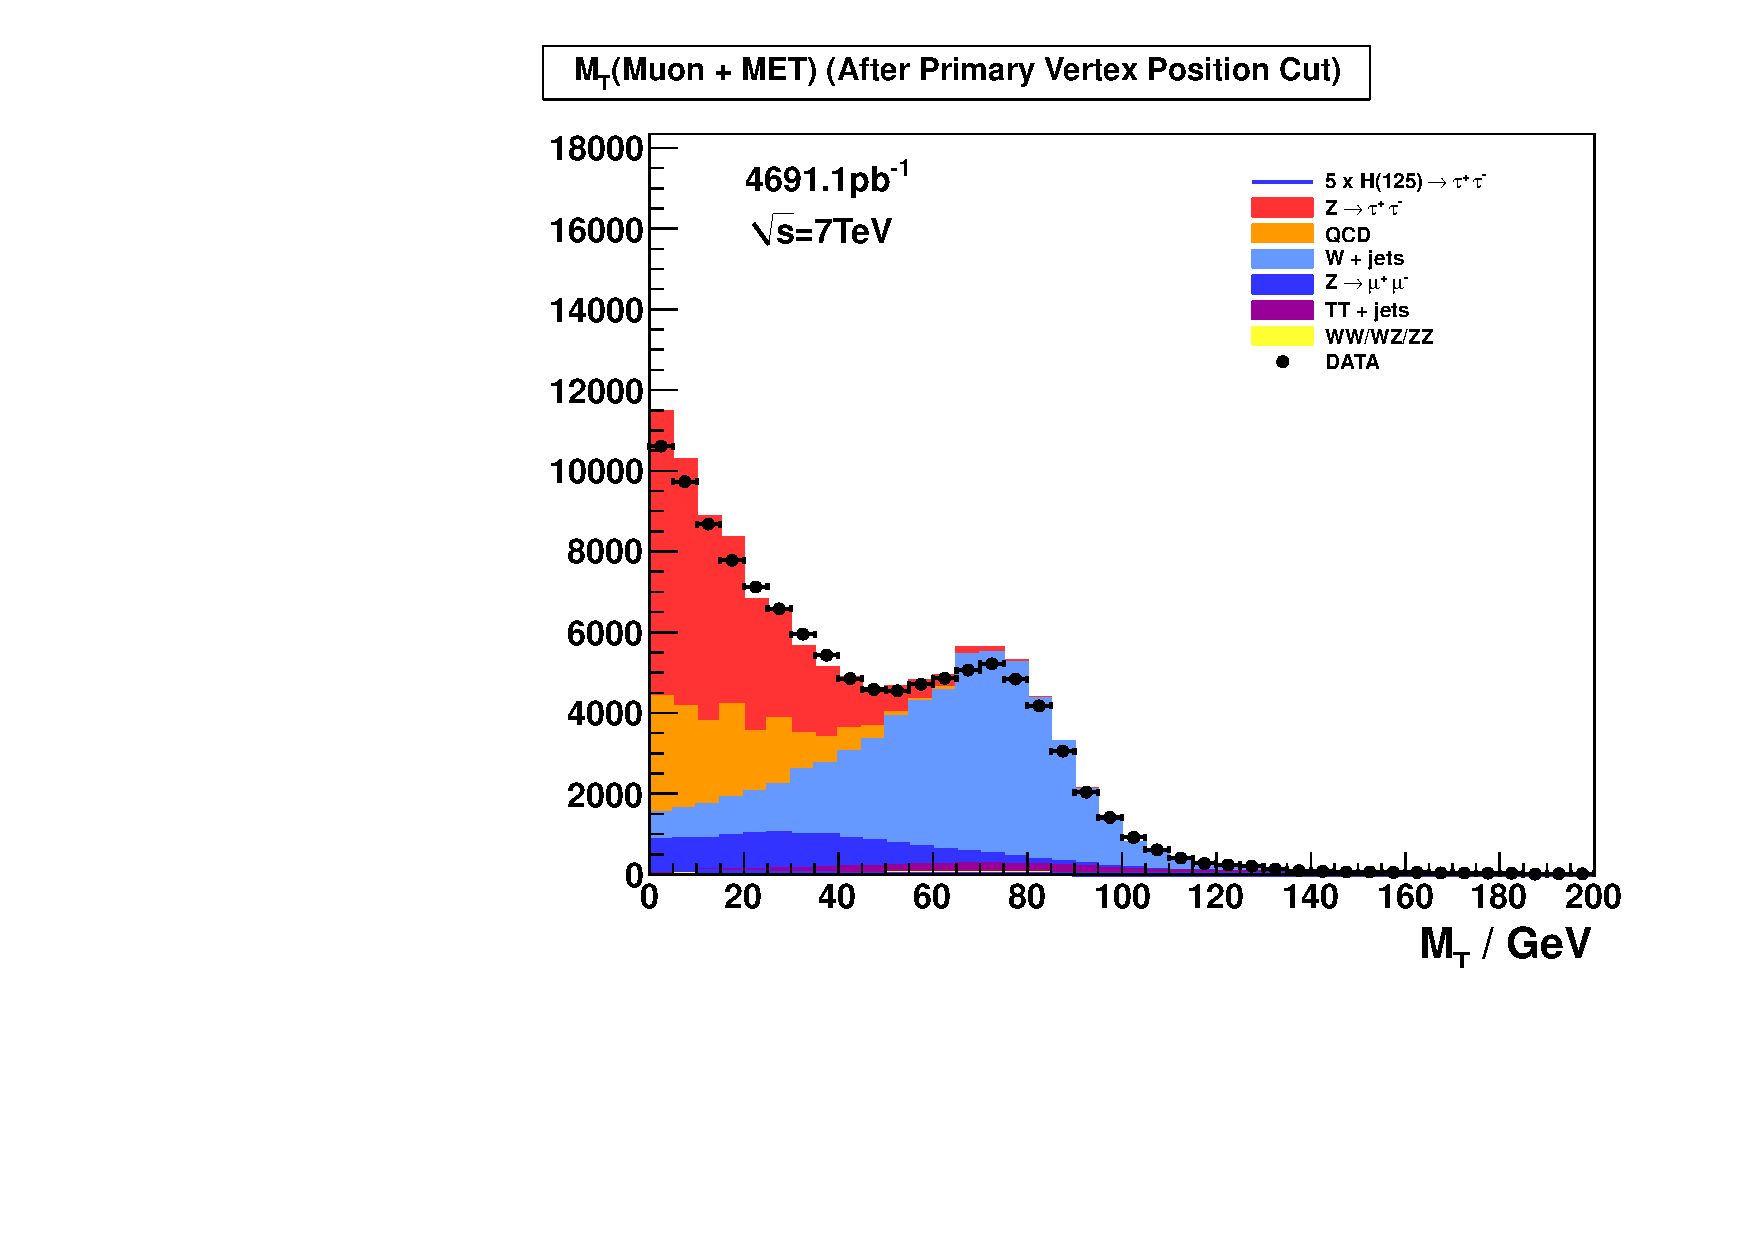
\includegraphics[scale=0.35]{plots/plotAHtoMuTau_leptonSelection_18_afterEvtSelPrimaryEventVertexPositionForMuTau_beforeEvtSelDiTauCandidateForMuTauMt1MET_mtMuonMET_linear.pdf}
\end{minipage}
\hspace{0.5cm}
\begin{minipage}[b]{0.5\linewidth}
\centering
  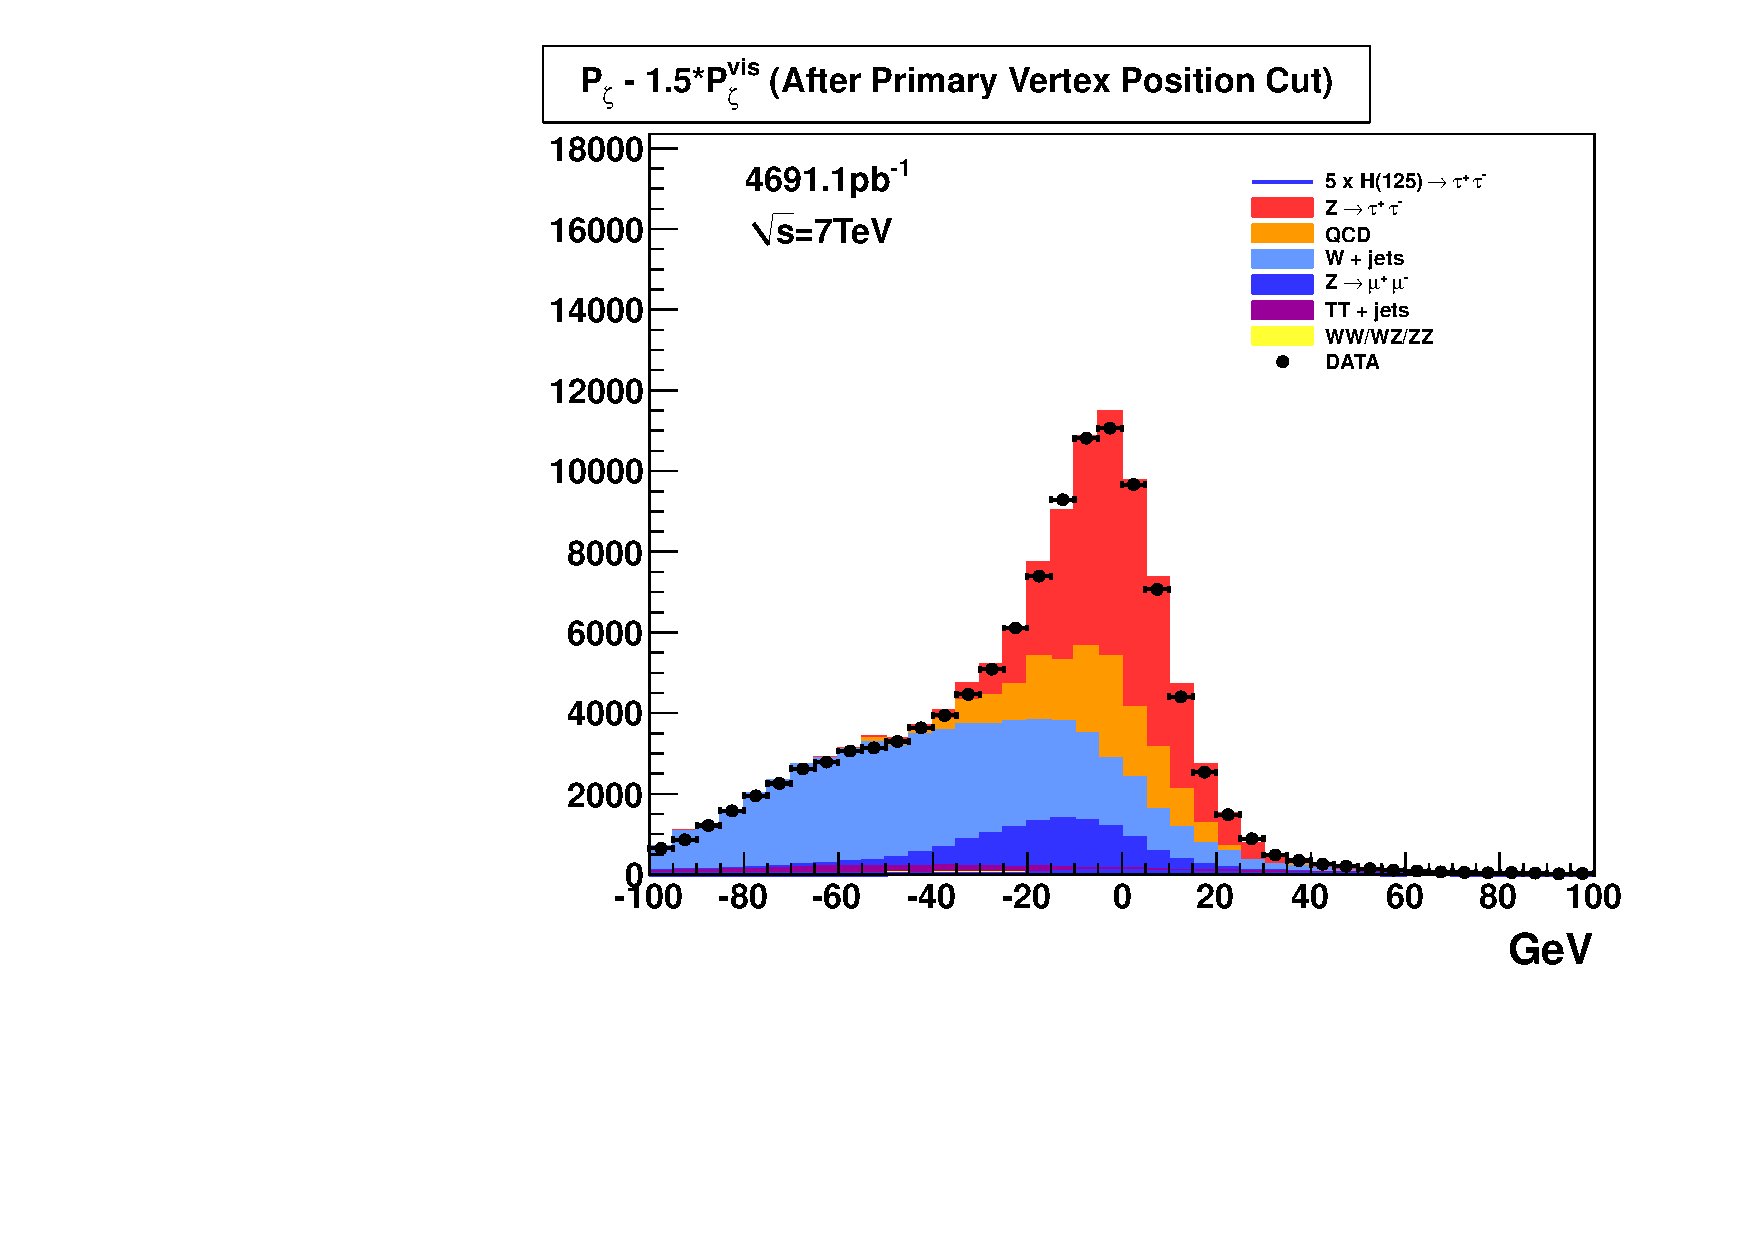
\includegraphics[scale=0.35]{plots/plotAHtoMuTau_leptonSelection_18_afterEvtSelPrimaryEventVertexPositionForMuTau_beforeEvtSelDiTauCandidateForMuTauMt1MET_PzetaDiff_linear}
\end{minipage}
\caption{$M_{T}$ and $\pzetadiff$ distributions.}
\label{fig:mtpzeta}
\end{figure}


In order to reject events arising from $Z \rightarrow \mu^{-}\mu^{+}$ an event is rejected based on the existence of a second loosely selected muon.
The second loosely selected muon is defined as a muon that has a track in the inner tracker matched to a track in the muon system, a  $p_{T} > 15$ GeV, $-2.4 < \eta < 2.4$, and $I_{rel} < 0.15$.
Once a collection of loosely selected muons is compiled the loosely selected muons are matched to muons selected as in Section \ref{sec:muonselection} using a maximum distance ($\Delta R$) in $\eta-\phi$ space of $0.5$.
An event is rejected if there are any matched muon pairs found in the event.
A similar procedure is repeated again in order to reduce backgrounds arising from the production of $Z/\gamma^{*} \rightarrow \mu^{-}\mu^{+}$.
This second di-muon rejection is performed with muons that satisfy the previous selection with the exception that the second muon does not have the $p_{T}$ and $I_{rel}$ requirements, additionally the di-muon pair is required to have zero charge and match within $\Delta R < 1.0$.


Finally since the Higgs bosons in question are neutral, a cut is applied such that the the muon and tau are required to have opposite charge.
The invariant mass of the visible tau lepton decay products before the $W$ boson discrimination, before the di-muon veto, and after the di-muon veto can be seen in Figure \ref{fig:mvisible}.
\begin{figure}[ht]
\centering
\includeditauplot{leptonSelection}{18_afterEvtSelPrimaryEventVertexPositionForMuTau_beforeEvtSelDiTauCandidateForMuTauMt1MET}{mVisible}{linear}
%\includeditauplot{leptonSelection}{18_afterEvtSelPrimaryEventVertexPositionForMuTau_beforeEvtSelDiTauCandidateForMuTauMt1MET}{mVisible}{linear}

\includeditauplot{sm}{19_afterEvtSelDiTauCandidateForMuTauMt1MET_beforeEvtSelDiMuPairZmumuHypothesisVetoByLooseIsolation}{mVisible}{linear}
%\includeditauplot{mssm}{19_afterEvtSelDiTauCandidateForMuTauPzetaDiff_beforeEvtSelDiMuPairZmumuHypothesisVetoByLooseIsolation}{mVisible}{linear}
\includefinalditauplot{zeroJets}{21_afterEvtSelDiMuPairDYmumuHypothesisVeto_beforeEvtSelJetEtCut}{mVisible}{linear}
%\includeditauplot{mssm}{21_afterEvtSelDiMuPairDYmumuHypothesisVeto_beforeEvtSelJetEtCut}{mVisible}{linear}

\caption{Invariant mass of visible tau decay products before the $W$ and $Z\rightarrow\mu\mu$ rejection (top), after the $W$ rejection (bottom left) and after the $Z\rightarrow\mu\mu$ rejection (bottom right) cuts.}
\label{fig:mvisible}
\end{figure}


\subsection{Secondary Vertex Fit}
\label{sec:nsvfit}
In order to extract the signal the invariant mass, $m_{\tau\tau}$, of the di-tau pair is fully reconstructed using a secondary vertex fit algorithm. % No Reference \cite{SVFIT}.
The algorithm performs a maximum likelihood fit taking input variables from the muon/tau four-momenta and the $\met$.
The variables to be fit for are the opening angle $\theta$ between the tau lepton and the visible momentum vector, the azimuthal angle $\overline\phi$ of the tau lepton with respect to the visible momentum vector in the laboratory frame, and the neutrino invariant mass $m_{\nu\nu}$.
The tau decay vertex (secondary vertex) is measured and an additional constraint is applied using the probability for a tau lepton to decay within the distance measured.
%(FIXME used?).
%(FIXME MORE!!!).


\subsection{Standard Model and MSSM Event Categories}
\label{sec:categories}
Events will be categorized based on the number of jets that satisfy requirements based on the jet(s) $p_{T}$, B-Tagging, and the jet(s) pseudo-rapidity.
The following standard model categories are defined according to the jet content of the event:
\begin{itemize}
\item \emph{Zero/One Jet}: This event category is designed to select events originating from the production mechanism in which the Higgs is produced via gluon-gluon fusion.
  It has the requirement that a maximum of one selected jet with $p_{T} > 30$ GeV and $-4.5 < \eta < 4.5$ is allowed.
  Secondly, in order to disallow any overlap between event categories, an event will fail to enter this category if it contains a jet with $p_{T} > 150$ GeV.
\item \emph{Boost}: This event category is designed to capture events in which the Higgs boson is highly boosted due to initial state radiation, or when produced in association with a W(Z) boson or top quark.
This category leverages the existence of a high $p_{T}$ jet recoiling from the boosted Higgs boson. 
As such the category requires a jet with $p_{T} > 150$ GeV.
%  This leads to the requirement that at least one jet must exist in the event with $p_{T} > 150$ GeV.
\item \emph{VBF}: This event category is designed to select events with the unique signature associated with vector boson fusion.
  In this category two jets with $p_{T} > 30$ GeV are required, each being located in the different hemispheres of the detector.
  Finally it is required that those jets are separated by $\Delta\eta > 4.0$ with no other selected jets between the leading jets in $\eta$.
\end{itemize}

As the MSSM Higgs has modified production mechanisms, the following categories are defined according to the jet content of the event:
\begin{itemize}
\item \emph{Non B-Tag}: This event category is designed to select events arising from the most prominent MSSM Higgs boson production mechanism of gluon-gluon fusion.
  It requires there to be no more than a single jet with $p_{T} > 30$ GeV and $-4.5 < \eta < 4.5$ while requiring zero jets with $p_{T} > 20$ GeV that meet B-Tag requirements.
\item \emph{B-Tag}: This event category is designed to leverage the MSSM Higgs boson production mechanism in association with b-quarks.
  It requires there to be no more than a single jet with $p_{T} > 30$ GeV and $-4.5 < \eta < 4.5$ while also requiring at least one jet with $p_{T} > 20$ GeV that meet B-Tag requirements.
\end{itemize}
The lepton kinematic distributions after the final event selection for \zeroJets, \boosted, \vbf, \wBtag, and \woBtag, can be seen in Figures \ref{fig:finalleptonzerojets}, \ref{fig:finalleptonboosted}, \ref{fig:finalleptonvbf}, \ref{fig:finalleptonwobtag}, and \ref{fig:finalleptonwbtag} respectively.
The reconstructed mass distribution for the SM categories \zeroJets, \boosted, and \vbf, can be seen in Figures \ref{fig:smmasszerojets}, \ref{fig:smmassboosted}, \ref{fig:smmassvbf}. 
The reconstructed mass distributions for the MSSM categories \woBtag, and \wBtag, can be seen in Figures \ref{fig:mssmmasswobtag}, and \ref{fig:mssmmasswbtag}.



% zeroJets
\begin{figure}[ht]
\includeleptonplot{zeroJets}{muon}{Pt}{log}
%\hspace{0.5cm}
\includeleptonplot{zeroJets}{tau}{Pt}{log}

\includeleptonplot{zeroJets}{muon}{Eta}{linear}
%\hspace{0.5cm}
\includeleptonplot{zeroJets}{tau}{Eta}{linear}
%
%\includeleptonplot{zeroJets}{muon}{Phi}{linear}
%\hspace{0.5cm}
%\includeleptonplot{zeroJets}{tau}{Phi}{linear}
%
\caption{Final selected $p_{T}$ (top) and $\eta$ (bottom) distributions for muons (left) and  taus (right) for the \emph{Zero/One Jets} category.}
\label{fig:finalleptonzerojets}
\end{figure}

% boosted
\begin{figure}[ht]
\includeleptonplot{boosted}{muon}{Pt}{linear}
%\hspace{0.5cm}
\includeleptonplot{boosted}{tau}{Pt}{linear}

\includeleptonplot{boosted}{muon}{Eta}{linear}
%\hspace{0.5cm}
\includeleptonplot{boosted}{tau}{Eta}{linear}
%
%\includeleptonplot{boosted}{muon}{Phi}{linear}
%\hspace{0.5cm}
%\includeleptonplot{boosted}{tau}{Phi}{linear}
%
\caption{Final selected $p_{T}$ (top) and $\eta$ (bottom) distributions for muons (left) and  taus (right) for the \emph{Boost} category.}
\label{fig:finalleptonboosted}
\end{figure}

% wVBFtag
\begin{figure}[ht]
\includeleptonplot{wVBFtag}{muon}{Pt}{linear}
\hspace{0.5cm}
\includeleptonplot{wVBFtag}{tau}{Pt}{linear}

\includeleptonplot{wVBFtag}{muon}{Eta}{linear}
%\hspace{0.5cm}
\includeleptonplot{wVBFtag}{tau}{Eta}{linear}
%
%\includeleptonplot{wVBFtag}{muon}{Phi}{linear}
%\hspace{0.5cm}
%\includeleptonplot{wVBFtag}{tau}{Phi}{linear}
%
\caption{Final selected $p_{T}$ (top) and $\eta$ (bottom) distributions for muons (left) and  taus (right) for the \emph{VBF} category.}
\label{fig:finalleptonvbf}
\end{figure}

% woBtag
\begin{figure}[ht]
\includeleptonplot{woBtag}{muon}{Pt}{log}
%\hspace{0.5cm}
\includeleptonplot{woBtag}{tau}{Pt}{log}

\includeleptonplot{woBtag}{muon}{Eta}{linear}
%\hspace{0.5cm}
\includeleptonplot{woBtag}{tau}{Eta}{linear}
%
%\includeleptonplot{woBtag}{muon}{Phi}{linear}
%\hspace{0.5cm}
%\includeleptonplot{woBtag}{tau}{Phi}{linear}
%
\caption{Final selected $p_{T}$ (top) and $\eta$ (bottom) distributions for muons (left) and  taus (right) for the \emph{Non B-Tag} category.}
\label{fig:finalleptonwobtag}
\end{figure}

% wBtag
\begin{figure}[ht]
\includeleptonplot{wBtag}{muon}{Pt}{linear}
%\hspace{0.5cm}
\includeleptonplot{wBtag}{tau}{Pt}{linear}

\includeleptonplot{wBtag}{muon}{Eta}{linear}
%\hspace{0.5cm}
\includeleptonplot{wBtag}{tau}{Eta}{linear}
%
%\includeleptonplot{wBtag}{muon}{Phi}{linear}
%\hspace{0.5cm}
%\includeleptonplot{wBtag}{tau}{Phi}{linear}
%
\caption{Final selected $p_{T}$ (top) and $\eta$ (bottom) distributions for muons (left) and  taus (right) for the \emph{B-Tag} category.}
\label{fig:finalleptonwbtag}
\end{figure}

%Mass SM
\begin{figure}[ht]
\includefullplot{zeroJets}{mSVmethod}{log}
\caption{Di-Tau invariant mass distribution in the \emph{Zero/One Jets} event category.}
\label{fig:smmasszerojets}
\end{figure}

\begin{figure}[ht]
\includefullplot{boosted}{mSVmethod}{linear}
\caption{Di-Tau invariant mass distributions in the \emph{Boost} event category.}
\label{fig:smmassboosted}
\end{figure}

\begin{figure}[ht]
\includefullplot{wVBFtag}{mSVmethod}{linear}
\caption{Di-Tau invariant mass distributions in the \emph{VBF} event category.}
\label{fig:smmassvbf}
\end{figure}

%Mass MSSM
\begin{figure}[ht]
\includefullplot{woBtag}{mSVmethod}{log}

\caption{Di-Tau invariant mass distributions in the \emph{Non B-Tag} event category.}
\label{fig:mssmmasswobtag}
\end{figure}

\begin{figure}[ht]
\includefullplot{wBtag}{mSVmethod}{linear}

\caption{Di-Tau invariant mass distributions in the \emph{B-Tag} event category.}
\label{fig:mssmmasswbtag}
\end{figure}



